% TikZ diagram gallery -- demonstration project
% Compile with: latexmk -pdf main.tex
\documentclass[a4paper,10pt]{article}
\usepackage[a4paper,landscape,margin=1.4cm,top=1.5cm,bottom=1.3cm]{geometry}
\usepackage[T1]{fontenc}
\usepackage[utf8]{inputenc}
\usepackage{amsmath,amssymb}
\usepackage{newpxtext,newpxmath}
\usepackage{microtype}
\usepackage{xcolor}
\usepackage{tikz}
\usetikzlibrary{arrows.meta,calc,positioning,shapes.geometric,fit,backgrounds,angles,quotes}
\usepackage{tikz-cd}

\definecolor{wine}{HTML}{7F1D1D}
\definecolor{ink}{HTML}{1C1917}
\definecolor{sea}{HTML}{1D4E89}
\definecolor{moss}{HTML}{2F6B3A}
\definecolor{ochre}{HTML}{B7791F}
\definecolor{paper}{HTML}{FBF7EE}
\definecolor{sand}{HTML}{F3ECDA}
\definecolor{line}{HTML}{DDD2B8}

\pagecolor{paper}
\color{ink}
\pagestyle{empty}
\setlength{\parindent}{0pt}

\newcommand{\panel}[3]{% title, height, content
  \begin{minipage}[t]{0.322\textwidth}
    {\scshape\color{wine}\small #1}\par\vspace{2pt}
    {\color{line}\hrule height 0.6pt}\vspace{6pt}
    \begin{minipage}[c][#2][c]{\linewidth}\centering #3\end{minipage}
  \end{minipage}%
}

\tikzset{
  >={Stealth[length=2mm]},
  every node/.style={font=\footnotesize},
  nn/.style={circle,draw=ink!70,thick,minimum size=5.2mm,inner sep=0pt,fill=white},
  box/.style={rounded corners=2pt,draw=ink!70,thick,fill=sand,minimum height=7mm,minimum width=20mm,align=center},
  dec/.style={diamond,aspect=2.2,draw=wine,thick,fill=white,align=center,inner sep=1pt},
  term/.style={rounded corners=8pt,draw=ink!70,thick,fill=white,minimum height=6mm,minimum width=14mm},
}

\begin{document}

\begin{minipage}[b]{0.7\textwidth}
  {\Huge\bfseries TikZ diagram gallery}\\[2pt]
  {\large\itshape Six vector figures, drawn in pure \LaTeX{} --- no images, no external tools.}
\end{minipage}\hfill
\begin{minipage}[b]{0.28\textwidth}\raggedleft\small
  Demonstration project\\
  TikZ \textperiodcentered{} PGF \textperiodcentered{} tikz-cd
\end{minipage}

\vspace{4pt}{\color{wine}\hrule height 1.2pt}\vspace{10pt}

\panel{1 \quad Neural network}{6.9cm}{%
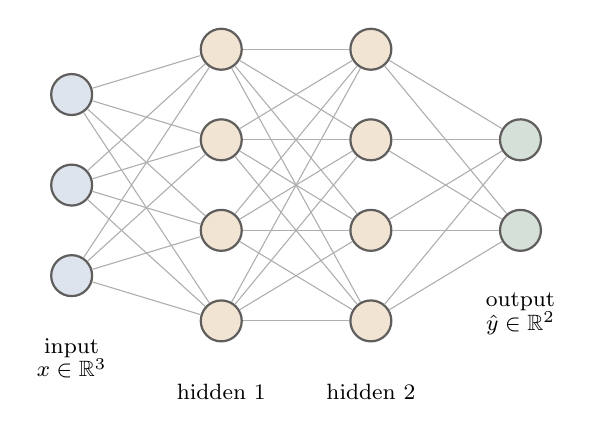
\begin{tikzpicture}[x=1.9cm,y=1cm]
  \foreach \i in {1,2,3} { \node[nn,fill=sea!15] (i\i) at (0,{(2-\i)*1.15+0}) {}; }
  \foreach \j in {1,2,3,4} { \node[nn,fill=ochre!20] (h\j) at (1,{(2.5-\j)*1.15}) {}; }
  \foreach \k in {1,2,3,4} { \node[nn,fill=ochre!20] (g\k) at (2,{(2.5-\k)*1.15}) {}; }
  \foreach \l in {1,2} { \node[nn,fill=moss!20] (o\l) at (3,{(1.5-\l)*1.15}) {}; }
  \foreach \i in {1,2,3} \foreach \j in {1,2,3,4} \draw[ink!35] (i\i) -- (h\j);
  \foreach \j in {1,2,3,4} \foreach \k in {1,2,3,4} \draw[ink!35] (h\j) -- (g\k);
  \foreach \k in {1,2,3,4} \foreach \l in {1,2} \draw[ink!35] (g\k) -- (o\l);
  \node[below=4mm of i3,align=center] {input\\[-1pt]$x\in\mathbb{R}^3$};
  \node[below=1mm of h4,align=center,yshift=-3mm] {hidden 1};
  \node[below=1mm of g4,align=center,yshift=-3mm] {hidden 2};
  \node[below=4mm of o2,align=center] {output\\[-1pt]$\hat y\in\mathbb{R}^2$};
\end{tikzpicture}}
\hfill
\panel{2 \quad Flowchart}{6.9cm}{%
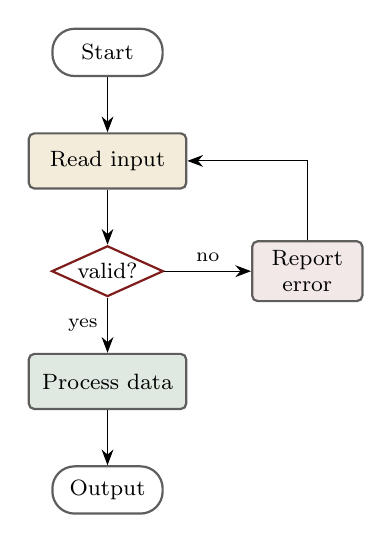
\begin{tikzpicture}[node distance=7mm]
  \node[term] (s) {Start};
  \node[box,below=of s] (r) {Read input};
  \node[dec,below=of r] (v) {valid?};
  \node[box,below=of v,fill=moss!15] (p) {Process data};
  \node[term,below=of p] (e) {Output};
  \node[box,right=11mm of v,fill=wine!10,minimum width=14mm] (x) {Report\\error};
  \draw[->] (s) -- (r);
  \draw[->] (r) -- (v);
  \draw[->] (v) -- node[left,font=\scriptsize] {yes} (p);
  \draw[->] (p) -- (e);
  \draw[->] (v) -- node[above,font=\scriptsize] {no} (x);
  \draw[->] (x) |- ($(r.east)+(3mm,0)$) -- (r.east);
\end{tikzpicture}}
\hfill
\panel{3 \quad Triangle centres and Euler line}{6.9cm}{%
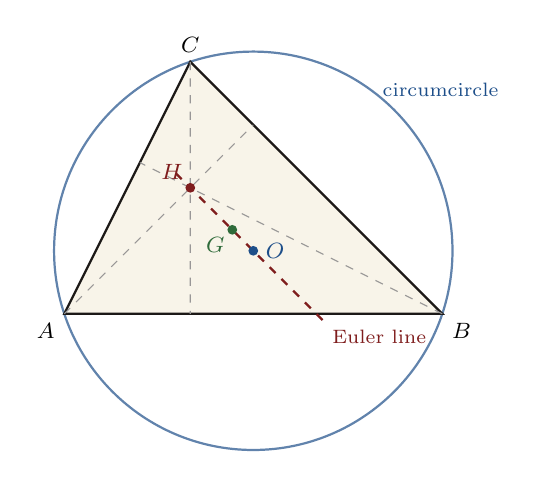
\begin{tikzpicture}[scale=0.8]
  \coordinate (A) at (0,0);
  \coordinate (B) at (6,0);
  \coordinate (C) at (2,4);
  \coordinate (O) at (3,1);
  \coordinate (G) at (8/3,4/3);
  \coordinate (H) at (2,2);
  \pgfmathsetmacro{\R}{sqrt(10)}
  \draw[sea!70,thick] (O) circle[radius=\R];
  \draw[ink,thick,fill=sand,fill opacity=0.6] (A) -- (B) -- (C) -- cycle;
  \draw[ink!45,dashed] (C) -- (2,0) (A) -- ($(B)!(A)!(C)$) (B) -- ($(A)!(B)!(C)$);
  \draw[wine,thick,dashed] ($(O)!-1.1!(H)$) -- ($(H)!-0.25!(O)$);
  \foreach \p/\pos in {A/below left,B/below right,C/above} \node[\pos] at (\p) {$\p$};
  \fill[sea] (O) circle (2.2pt) node[right=1pt] {$O$};
  \fill[moss] (G) circle (2.2pt) node[below left=-1pt] {$G$};
  \fill[wine] (H) circle (2.2pt) node[above left=-1pt] {$H$};
  \node[font=\scriptsize,sea,anchor=west] at (4.9,3.55) {circumcircle};
  \node[font=\scriptsize,wine,anchor=north west] at ($(O)!-1.1!(H)$) {Euler line};
\end{tikzpicture}}

\vspace{12pt}

\panel{4 \quad Commutative diagrams}{6.9cm}{%
\large
\begin{tikzcd}[row sep=huge,column sep=huge,ampersand replacement=\&]
  A \arrow[r,"f"] \arrow[d,"g"'] \arrow[dr,"h" description,color=wine] \& B \arrow[d,"p"] \\
  C \arrow[r,"q"'] \& D
\end{tikzcd}\\[14pt]
\begin{tikzcd}[column sep=small,ampersand replacement=\&]
  0 \arrow[r] \& A \arrow[r,"\iota",hook] \& B \arrow[r,"\pi",two heads] \& C \arrow[r] \& 0
\end{tikzcd}\\[4pt]
\normalsize{\footnotesize\itshape $p\circ f = q\circ g = h$ \quad and \quad $\ker\pi=\operatorname{im}\iota$}}
\hfill
\panel{5 \quad The unit circle}{6.9cm}{%
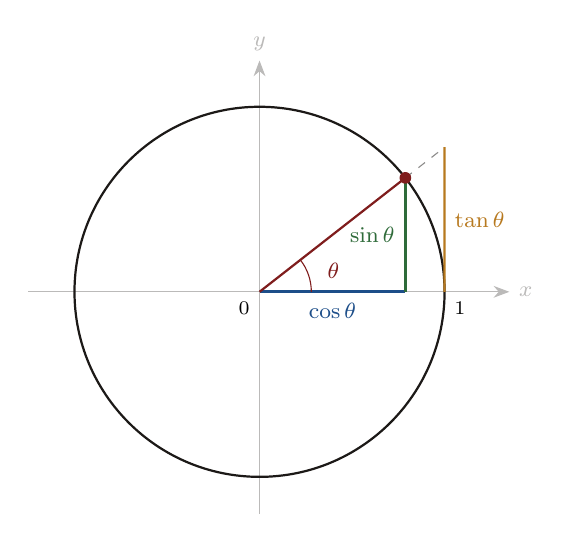
\begin{tikzpicture}[scale=2.35]
  \def\a{38}
  \draw[ink!30,->] (-1.25,0) -- (1.35,0) node[right] {$x$};
  \draw[ink!30,->] (0,-1.2) -- (0,1.25) node[above] {$y$};
  \draw[ink,thick] (0,0) circle (1);
  \coordinate (P) at ({cos(\a)},{sin(\a)});
  \coordinate (X) at ({cos(\a)},0);
  \coordinate (T) at (1,{tan(\a)});
  \draw[sea,very thick] (0,0) -- (X) node[midway,below] {$\cos\theta$};
  \draw[moss,very thick] (X) -- (P) node[midway,left] {$\sin\theta$};
  \draw[wine,thick] (0,0) -- (P);
  \draw[ochre,thick] (1,0) -- (T) node[midway,right] {$\tan\theta$};
  \draw[ink!50,dashed] (P) -- (T);
  \fill[wine] (P) circle (0.9pt);
  \draw[wine] (0.28,0) arc (0:\a:0.28);
  \node[wine] at (0.40,0.115) {$\theta$};
  \node[below left,font=\scriptsize] at (0,0) {$0$};
  \node[below right,font=\scriptsize] at (1,0) {$1$};
\end{tikzpicture}\\[-2pt]
{\footnotesize\itshape $\cos^2\theta+\sin^2\theta=1$}}
\hfill
\panel{6 \quad Shortest path (Dijkstra)}{6.9cm}{%
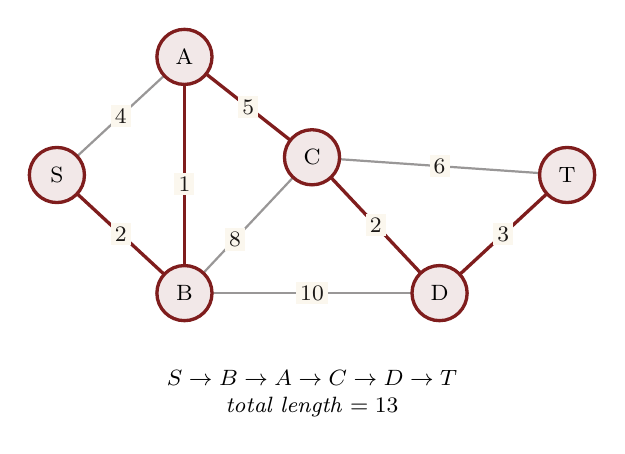
\begin{tikzpicture}[x=1.62cm,y=1.5cm,
  v/.style={circle,draw=ink!70,thick,fill=white,minimum size=7mm,inner sep=0pt},
  e/.style={ink!45,thick},
  w/.style={midway,fill=paper,inner sep=1.5pt,font=\footnotesize,text=ink},
  best/.style={wine,very thick}]
  \node[v] (S) at (0,1) {S};
  \node[v] (A) at (1,2) {A};
  \node[v] (B) at (1,0) {B};
  \node[v] (C) at (2,1.15) {C};
  \node[v] (D) at (3,0) {D};
  \node[v] (T) at (4,1) {T};
  \draw[e] (S) -- node[w] {4} (A);
  \draw[best] (S) -- node[w] {2} (B);
  \draw[best] (B) -- node[w,pos=.45] {1} (A);
  \draw[best] (A) -- node[w] {5} (C);
  \draw[e] (B) -- node[w,pos=.35] {8} (C);
  \draw[e] (B) -- node[w] {10} (D);
  \draw[best] (C) -- node[w] {2} (D);
  \draw[e] (C) -- node[w] {6} (T);
  \draw[best] (D) -- node[w] {3} (T);
  \foreach \n in {S,B,A,C,D,T} \node[v,draw=wine,very thick,fill=wine!10] at (\n) {\n};
  \node[align=center,font=\footnotesize\itshape] at (2,-0.85) {$S\to B\to A\to C\to D\to T$\\ total length $=13$};
\end{tikzpicture}}

\vfill
{\color{line}\hrule height 0.6pt}\vspace{4pt}
{\footnotesize\color{ink!70} Source: \texttt{main.tex} \textperiodcentered{} compiled with \texttt{latexmk -pdf} \textperiodcentered{} fonts: Palatino (newpx) \hfill N'sol\'e Samson Yamontche \textperiodcentered{} \LaTeX{} \& TikZ}

\end{document}

